\section{Autler-Townes Effect in a Superconducting Three-Level System \cite{PhysRevLett..193601}\label{sec:autlerEffectThreeLevelSystem}}
% Phase qubit is used, which is a JJ in series with an inductor. The JJ has its own effective capacitance and inductance. In this system:
% \begin{itemize}
% 	\item \textbf{Chraging energy} \ra kinetic energy;
% 	\item \textbf{Inductance energy} \ra $  E_{\text{potential}} = E_J(1-\cos(\phi_\text{JJ}))+\frac{\Phi_L^2}{2L_L} $;
% \end{itemize}
%
% \begin{table}[h]
% 	\centering
% 	\begin{tabular}{|c|c|c|}\hline
% 		External & JJ & Inductor\\\hline
% 		$ \Phi_\text{ext} $ & $ \Phi_\text{JJ} $ & $ \Phi_\text{L} $\\
% 		$ \phi_\text{ext} $ & $ \phi_\text{JJ} $ & $ \phi_\text{L} $\\
% 		& L\isub{JJ} & L\isub{L}\\
% 		& $ E_J\big(1-\cos(\phi_{\text{JJ}})\big) $ & $ \frac{\Phi_L^2}{2L_L} $\\\hline
% 	\end{tabular}
% \end{table}
% 
% \noindent \alert{Remembering that: a) $\phi = \frac{\Phi}{\Phi_0}2\pi$; b) $\Phi_\text{ext} + \Phi_\text{JJ} + \Phi_L = n\Phi_0$ (from the quantisation of flux inside a superconducting loop) and we use $ n=0 $}
% 
% \blue{\begin{equation}
% 	\label{l3-energy1}
% 	\begin{aligned}
% 	E(\phi_\text{JJ})_{\text{potential}} & = E_J\big(1-\cos(\phi_\text{JJ})\big) + \bigg(-\Phi_\text{ext} - \Phi_\text{JJ}\bigg)^2/2L_L\\
% 	&= E_J\big(1-\cos(\phi_\text{JJ})\big) + \bigg(\Phi_0\frac{(\phi_\text{ext}+\phi_\text{JJ})}{2\pi}\bigg)^2/{2L_L}\\
% 	& = E_J\big(1-\cos(\phi_\text{JJ})\big) + E_L{(\phi_\text{ext}+\phi_\text{JJ})^2}\\
% 	\end{aligned}
% 	\end{equation}}
% 
% \noindent which is a function of $\phi_J$. The second term gives a parabolic energy relation, while the first gives oscillations on this parabola (small wiggles) in Fig.\ref{fig:phij}. 
% 
% 
% \begin{figure}[h]
% 	\begin{center}
% 		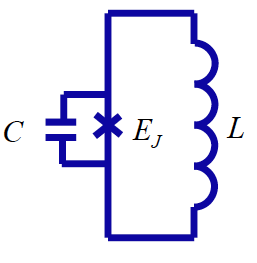
\includegraphics[height=3cm]{rf}
% 	\end{center}
% 	\caption{RF SQUID induction components.}
% 	\label{fig:rf}
% \end{figure}
% \begin{figure}[h]
% 	\ipic{5cm}{phij}
% 	\caption{Potential energy as a function of the external flux. 10 energy levels reside in each minima.}
% 	\label{fig:phij}
% \end{figure}
% 
% \noindent\textbf{Adding the charging energy} for a capacitor in parallel to the JJ (the effective kinetic energy term Eq.\ref{l3-energy1})
% \red{\[
% 	\begin{aligned}
% 	E_C& =\frac{Q^2}{2C} = E_C\hat{N}^2\\
% 	&\hat{N} \text{ was taken as canonical momentum } \hat{p} = -i\hbar\frac{d}{dx} \text{from which } \hat{N}=-i\frac{d}{d\phi}
% 	\end{aligned}
% 	\]}
% 
% \noindent one arrives at a Hamiltonian
% 
% \begin{equation}
% \label{l3-h1}
% \begin{aligned}
% \mathcal{H} & = \red{E_{с} \hat{N}^2} - \blue{E_J\cos(\phi_J) + E_L(\phi_\text{ext}+\phi_J)^2},\\
% \red{E_C = \frac{(2e)^2}{2C} }&\qquad\qquad\qquad \blue{E_L = \frac{\Phi_0^2}{(2\pi)^22L}}
% \end{aligned}
% \end{equation}
% 
% \red{\large So now one has a parabolic potential term in the Hamiltonian,}
% \begin{itemize}
% 	\item $ \phi_{\text{ext}} $ controls the shape of the potential and hence the energies of each eigenstate
% 	\item $ \phi_{\text{JJ}} $ is the dynamic parameter of the qubit - it changes to occupy potential wells etc.
% \end{itemize}
% 
% For solving numerically, we will work in the $ \ket{\phi_{\text{JJ}}} $ basis:
% 
%    {\large
% 	\begin{align}
% 	\left[\blue{x},\red{p}\right] & =i\hbar & \left[\blue{\Phi},\red{Q}\right] & = i\hbar & \left[\phi,N\right] & = \frac{2\pi}{\frac{h}{2e}}\left[\Phi,Q\right]\frac{1}{2e} = i\\
% 	 \red{\hat{p}} & = -i\hbar\ipartial{}{\blue{x}} & \hat{\red{Q}} & =-i\hbar\ipartial{}{\blue{\Phi}} & \hat{\red{N}} & =-i\ipartial{}{\blue{\phi}}
% 	\end{align}
% }
%
% \noindent i.e. $ \hat{N}  $ and $ \hat{\phi} $ behave like position and momentum operators, so evaluating the $ \hat{N} $ operator in the phase basis
% 
%    \begin{equation}
% 		\begin{aligned}
% 		\hat{N} &= -i\frac{1}{\Delta \phi_\text{JJ}}\sum\ketbra{\phi_\text{JJ} + 1}{\phi_\text{JJ}} + \ketbra{\phi_\text{JJ} - 1}{\phi_\text{JJ}}\\
% 		\hat{N}^2 &= -\frac{1}{\Delta \phi_\text{JJ}^2}\bigg[\sum\ketbra{\phi_\text{JJ} + 1}{\phi_\text{JJ}} + \ketbra{\phi_\text{JJ} - 1}{\phi_\text{JJ}}\bigg]\bigg[\sum\ketbra{\phi_\text{JJ} + 1}{\phi_\text{JJ}} + \ketbra{\phi_\text{JJ} - 1}{\phi_\text{JJ}}\bigg]\\
% 		\end{aligned}
% \end{equation}
% 
% \begin{equation}
% \begin{aligned}
% 	\hat{H} &= \red{E_c\sum_{\phi_{\text{JJ}}} \frac{1}{\Delta\phi_{\text{JJ}}^2} \ketbra{\phi_{\text{JJ}}}{\phi_{\text{JJ}}} 
% 			- \frac{1}{\Delta\phi_{\text{JJ}}^2} \ketbra{\phi_{\text{JJ}}+\Delta\phi_{\text{JJ}}}{\phi_{\text{JJ}}}  -
% 			- \frac{1}{\Delta\phi_{\text{JJ}}^2} \ketbra{\phi_{\text{JJ}}-\Delta\phi_{\text{JJ}}}{\phi_{\text{JJ}}}	}	
% \\ &\quad\quad \blue{\bigg[E_J\cos(\phi_{\text{JJ}}) + E_L(\phi_\text{ext}+\phi_J)^2\bigg]\sum_{\phi_{\text{JJ}}}\ketbra{\phi_{\text{JJ}}}{\phi_{\text{JJ}}}}
% \end{aligned}
% \end{equation}
% 
% \noindent or in matrix form (showing same arbitrary three elements in phase space)
%{\tiny  
%  \begin{equation}
%  \kbordermatrix{
% 	& \ket{\phi_{\text{JJ}}-\Delta\phi_{\text{JJ}}} & \ket{\phi_{\text{JJ}}} & \ket{\phi_{\text{JJ}}+\Delta\phi_{\text{JJ}}} \\
% 	\bra{\phi_{\text{JJ}}-\Delta\phi_{\text{JJ}}} & \red{\frac{E_c}{\Delta\phi_{\text{JJ}}^2}} + \blue{E_J\cos(\phi_{\text{JJ}} - \Delta\phi_{\text{JJ}}) + E_L(\phi_\text{ext}+\phi_{\text{JJ}}-\Delta\phi_{\text{JJ}})^2} & \red{-\frac{E_c}{2\Delta\phi_{\text{JJ}}^2}} & 0 \\
% 	\bra{\phi_{\text{JJ}}} & \red{-\frac{E_c}{2\Delta\phi_{\text{JJ}}^2}} & \red{\frac{E_c}{\Delta\phi_{\text{JJ}}^2}} + \blue{E_J\cos(\phi_{\text{JJ}}) + E_L(\phi_\text{ext}+\phi_J)^2} & \red{-\frac{E_c}{2\Delta\phi_{\text{JJ}}^2}}\\
% 	\bra{\phi_{\text{JJ}}+\Delta\phi_{\text{JJ}}} & 0 & \red{-\frac{E_c}{2\Delta\phi_{\text{JJ}}^2}} & \red{\frac{E_c}{\Delta\phi_{\text{JJ}}^2}} + \blue{E_J\cos(\phi_{\text{JJ}} + \Delta\phi_{\text{JJ}}) + E_L(\phi_\text{ext}+\phi_{\text{JJ}} + \Delta\phi_{\text{JJ}})^2}
% 	\\ }
% \end{equation}
% }
% If one plots the eigenfunctions as functions of the flux on the JJ $\phi_J$ and overlays them onto the plot of the potential, then one will have something of the form shown in Fig.\ref{fig:l3-myone}. Run the code \verb|RF_SQUID_1| to see the evolution.
% 
% 
%  The two eigenstates of this equation with the lowest energies \iket{0} and \iket{1} constitute to the two circulating current directions. The two eigenfunctions exits in the double well potential minimuma.
%   
   The system state is read out using the flux pulse method - applying  flux pulse changes the potential of the system, and state \iket{1} for example would be brought to the top of the `dip', allowing the system to tunnel out, change the phase across the JJ, which is registered by a SQUID
   
   \ipicCaption{4cm}{uPulse}{The $ \Delta U $ pulse excites the system from the well miniumum, allowing tunneling to occur from the lower levels.}
   
   As detailed in \verb|all_the_notes| a dark state is created when driving on resonance:
   
   \begin{equation}
   \begin{aligned}
   \red{E_0} &\red{= 0} & E_1 &= -\frac{\hbar}{2}\sqrt{\Omega_{21}^2+\Omega_{32}^2} & E_2 &= \frac{\hbar}{2}\sqrt{\Omega_{21}^2+\Omega_{32}^2}\\
   \red{\vec{v}_0} & \red{= \frac{1}{\sqrt{\Omega_{21}^2 + \Omega_{32}^2}}
   	\begin{pmatrix}
   	\Omega_{32}\\0\\-\Omega_{21}
   	\end{pmatrix}} & 
   \vec{v}_1  & =
   \begin{pmatrix}
   \Omega_{21}\\ -\sqrt{\Omega_{21}^2 + \Omega_{32}^2} \\ \Omega_{32}
   \end{pmatrix} &
   \vec{v}_2  & =
   \begin{pmatrix}
   \Omega_{21}\\ \sqrt{\Omega_{21}^2 + \Omega_{32}^2} \\ \Omega_{32}
   \end{pmatrix},\\
   \end{aligned}
   \end{equation}
 
   \noindent Now, as the \iket{1}\lra\iket{2} drive is increased, the dark state $  \cos(\Theta)\iket{0} - \sin(\Theta)\iket{2} $ is disturbed, as levels \iket{1} and \iket{2} begin to split. This allows relaxation to \iket{1} so the dark state is destroyed. Now that the population of \iket{1} is finite, we will register its' population (using the flux shift method as in Sec.~\ref{sec:coherentStateStorageBetweenPhaseQubits}) as a function of the \iket{0}\ra\iket{1} probe tone frequency.
  
   \ipic{5cm}{@AutlerTownesEffectThreeLevelSystem1}
   
   The splitting of level \iket{1} is induced by the strong control drive $ \Omega_c $:
   \[
   \varepsilon_{\pm} = \omega_{10} + \Delta_c/2 \pm \sqrt{\Delta_c^2+\Omega_c^2}/2,
   \]
   
   \noindent and at resonance of the control field, $ \Delta_c = 0 $, the splitting of level \iket{1} will be $ \Omega_c $ exactly. To see this, let us monitor the anticrossing:
   
   \ipicCaption{7.5cm}{@AutlerTownesEffectThreeLevelSystem2}{$ f_p \equiv \iket{0}\lra\iket{1}$ picks up the splitting of the \iket{1}. We see, that at resonance of the control field, the Rabi splitting is minimal, and then it deviates. \red{Nore that this is the mesured probability of \iket{1} and \iket{2} together, since it is hard to separate their populations using the flux shift readout method.}}
   
   
 \newpage
